\documentclass[a4paper,14pt]{extarticle}
\usepackage[utf8]{inputenc}
\usepackage[russian]{babel}
\usepackage{graphicx}
\usepackage[top=0.8in, bottom=0.8in, left=0.8in, right=0.8in]
{geometry}
\usepackage{pgfplots}
\usepackage{amsmath}
\usepackage{setspace}
\usepackage{titlesec}
\usepackage{float}
\usepackage{chngcntr}
\usepackage{pgfplots}
\usepackage{amsfonts}
\usepackage{pgfplotstable}
\usepackage{multirow}
\usepackage{karnaugh-map}
\usepackage{tikz,xcolor}
\usepackage{indentfirst} % Красная строка
\usepackage{listings}
\usepackage{amssymb}
\usepackage{xcolor}
\usepackage{hyperref}

\definecolor{linkcolor}{HTML}{0000FF} % цвет ссылок
\definecolor{urlcolor}{HTML}{FF00FF} % цвет гиперссылок

\hypersetup{pdfstartview=FitH, linkcolor=linkcolor,urlcolor=urlcolor, colorlinks=true}


\titleformat{\section}[hang]
  {\bfseries}
  {}
  {0em}
  {\hspace{-0.4pt}\large \thesection\hspace{0.6em}}
  
  
\titleformat{\subsection}[hang]
  {\bfseries}
  {}
  {0em}
  {\hspace{-0.4pt}\large \thesubsection\hspace{0.6em}}

%\linespread{1.3} % полуторный интервал
%\renewcommand{\rmdefault}{ftm} % Times New Roman

\newcommand{\nx}{\overline{x}}
\newcommand{\p}{0.31}
\newcommand{\scale}{1.4}

\counterwithin{figure}{section}
\counterwithin{equation}{section}
\counterwithin{table}{section}

\begin{document}
\begin{titlepage}
\centering
Санкт-Петербургский политехнический университет Петра Великого \\
\vspace{0.15cm}
Кафедра компьютерных систем и программных технологий \\
\vspace{6.5cm}

{\centering \textbf{Отчёт по лабораторной работе} \\ 
\vspace{0.15cm}
\textbf{Дисциплина}: Телекоммуникационные технологии \\
\vspace{0.15cm}
\textbf{Тема}: Аналоговая, частотная и фазовая модуляция.} \\


\vspace{6.5cm}

\begin{table}[H]
\begin{tabular}{p{\textwidth}@{}r}
{Выполнил студент гр. 33501/4} \hfill {Мальцев  М.С.} \\
{Преподаватель} \hfill {Богач Н.В.} \\
\end{tabular}
\end{table}
\vfill

{\centering Санкт-Петербург \\ 
\vspace{0.15cm}
\today}
\end{titlepage}

\tableofcontents

\newpage

\section{Цель работы}

Изучение амплитудной частотной и фазовой модуляции/демодуляции сигнала.

\section{Постановка задачи}

\begin{enumerate}
\item Сгенерировать однотональный сигнал низкой частоты.

\item Выполнить амплитудную модуляцию (АМ) сигнала по закону
$$ u(t) = (1 + MU_m cos(\Omega t)) cos(\omega_0 t + \phi_0)$$
для различных значений глубины модуляции M. Используйте встроенную функцию MatLab $ammod$.

Выполнить фазовую модуляцию/демодуляцию сигнала по закону 
$$ u(t) = U_m cos(\Omega t + ks(t)$$
используя встроенную функцию MatLab $pmmod$, $pmdemod$

\item Получить спектр модулированного сигнала.

\item Выполнить модуляцию с подавлением несущей.
$$ u(t) = MU_m cos(\Omega t) cos(\omega_0 t + \phi_0)$$
получить спектр.
\item Выполнить однополосную модуляцию:
$$\displaystyle u(t) = U_m cos(\Omega t) cos(\omega_0 t + \phi_0) + \frac{U_m}{2} \sum^N_{n=1}M_n(cos(\omega_0 + \Omega_n) t + \phi_0 + \Phi_n)$$
положив n=1.

\item Выполнить частотную модуляцию/демодуляцию по закону
$$\displaystyle u(t) = U_m cos(\omega_0 t + k \int_0^t s(t)dt + \phi_0)$$
используя встроенные функции MatLab $fmmod$, $fmdemod$.

\item Выполнить синхронное детектирование и получить исходный
однополосный сигнал.

\item Рассчитать КПД модуляции.
$$\displaystyle \eta_{AM} = \frac{U^2_m M^2/4}{P_U} = \frac{M^2}{M^2 + 2}$$
\end{enumerate}

\section{Теоретический раздел}

Модуляция — процесс изменения одного или нескольких параметров модулируемого несущего сигнала при помощи модулирующего сигнала.

В некоторых случаях параметры переносчика изменяются под действием модулирующей дискретной последовательности и принимают дискретные значения. Такой процесс называют манипуляцией в отличие от модуляции, при которой параметры переносчика изменяются непрерывно.

Если в качестве переносчика выбрано синусоидальное высокочастотное колебание, то реализуется аналоговая модуляция.

Если в качестве переносчика используется периодическая последовательность импульсов, основными параметрами которой являются амплитуда импульсов, длительность импульсов, их временное положение и частота следования, то можно получить следующие виды модуляции: амплитудно-импульсную (АИМ), широтно-импульсную (ШИМ), фазо-импульсную (ФИМ) и частотно-импульсную (ЧИМ). Следует иметь в виду, что импульсные способы модуляции не используются для передачи информации на большие расстояния. Поэтому когда говорят о системах с импульсной модуляцией, то имеется в виду двойная модуляция, т. е. модуляция импульсной последовательности исходным сообщением, а затем модуляция высокочастотного гармонического колебания импульсной последовательностью.

Обратные операции по восстановлению величин, вызвавших изменение параметров переносчика при модуляции, называются демодуляцией.\\\\
Использование модуляции позволяет:
\begin{itemize}
\item согласовать параметры сигнала с параметрами линии;
\item повысить помехоустойчивость сигналов;
\item увеличить дальность передачи сигналов;
\item организовать многоканальные системы передачи (МСП с ЧРК).\\
\end{itemize}
В качестве несущего сигнала может использоваться:
\begin{itemize}
\item гармоническое колебание, при этом модуляция называется аналоговой или непрерывной;
\item периодическая последовательность импульсов, при этом модуляция называется импульсной;
\item постоянный ток, при этом модуляция называется шумоподобной.\\
\end{itemize}

В зависимости от изменяемого параметра различают три основных вида модуляции – \textbf{амплитудную}, \textbf{частотную} и \textbf{фазовую}.

\subsection{Амплитудная модуляции}

Амплитудная модуляции -- вид модуляции, при которой изменяемым параметром несущего сигнала является его амплитуда.\\\\
Основными достоинствами амплитудной модуляции являются:
\begin{itemize}
\item узкая ширина спектра АМ сигнала;
\item простота получения модулированных сигналов.\\
\end{itemize}
Недостатками этой модуляции являются:
\begin{itemize}
\item низкая помехоустойчивость (т. к. при воздействии помехи на сигнал искажается его форма — огибающая, которая и содержит передаваемое сообщение);
\item неэффективное использование мощности передатчика (т. к. наибольшая часть энергии модулированного сигнала содержится в составляющей несущего сигнала до 64\%, а на информационные боковые полосы приходится по 18\%).\\
\end{itemize}
Амплитудная модуляция нашла широкое применение:
\begin{itemize}
\item в системах телевизионного вещания (для передачи телевизионных сигналов);
\item в системах звукового радиовещания и радиосвязи на длинных и средних волнах;
\item в системе трехпрограммного проводного вещания.
\end{itemize}

\begin{figure}[H]
\center{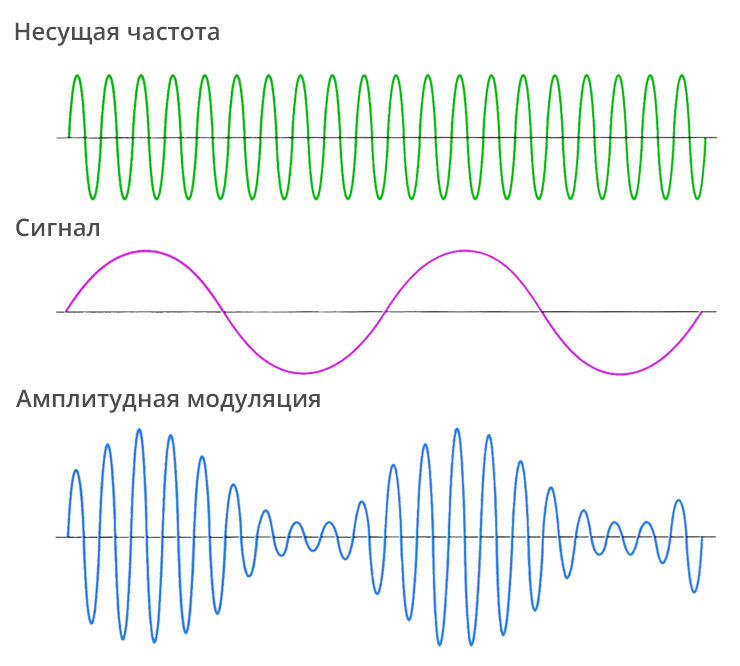
\includegraphics[width=0.5\linewidth]{img/100}}
\caption{Амплитудная модуляция}
\end{figure}

\subsection{Частотная модуляции}

При частотной модуляции изменяемым параметром несущего сигнала является его частота. Важной особенностью спектра ЧМ сигнала является то, что можно добиться отсутствия составляющей несущего сигнала или сделать ее амплитуду значительно меньше амплитуд информационных составляющих без дополнительных технических усложнений модулятора.\\\\
Достоинством частотной модуляции являются:
\begin{itemize}
\item высокая помехоустойчивость;
\item более эффективное использование мощности передатчика;
\item сравнительная простота получения модулированных сигналов.
\end{itemize}
Основным недостатком данной модуляции является большая ширина спектра модулированного сигнала.\\\\
Частотная модуляция используется:
\begin{itemize}
\item в системах телевизионного вещания (для передачи сигналов звукового сопровождения);
\item системах спутникового теле- и радиовещания;
\item системах высококачественного стереофонического вещания (FM диапазон);
\item радиорелейных линиях (РРЛ);
\item сотовой телефонной связи.\\
\end{itemize}

\begin{figure}[H]
\center{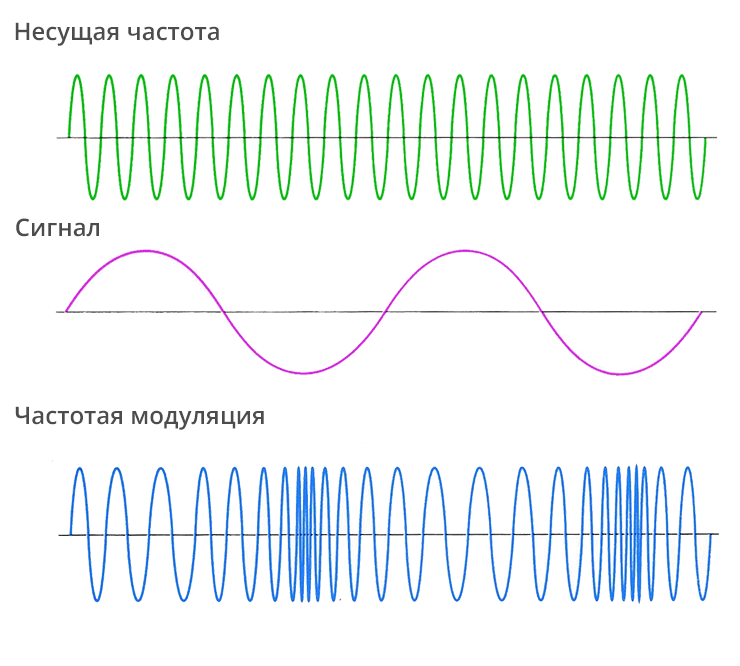
\includegraphics[width=0.48\linewidth]{img/101}}
\caption{Частотная модуляция}
\end{figure}

\subsection{Фазовая модуляции}

Фазовая модуляция -- один из видов модуляции колебаний, при которой фаза несущего колебания управляется информационным сигналом.\\\\
Достоинствами фазовой модуляции являются:
\begin{itemize}
\item высокая помехоустойчивость;
\item более эффективное использование мощности передатчика.\\
\end{itemize}
Недостатками фазовой модуляции являются:
\begin{itemize}
\item большая ширина спектра;
\item сравнительная трудность получения модулированных сигналов и их детектирование.\\
\end{itemize}

\begin{figure}[H]
\center{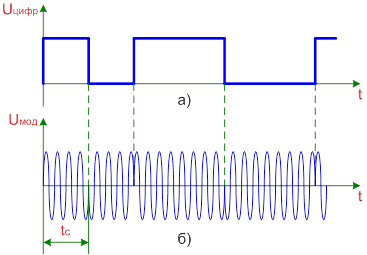
\includegraphics[width=0.7\linewidth]{img/102}}
\caption{Фазовая модуляция}
\end{figure}

\newpage

\section{Ход работы}

Была синтезирована схема, для моделирования синусоидального сигнала. 
Синтезированная схема представлена на рисунке \ref{000}, а результат симуляции на рисунке \ref{002}.

\begin{figure}[H]
\begin{minipage}[h]{0.49\linewidth}
\center{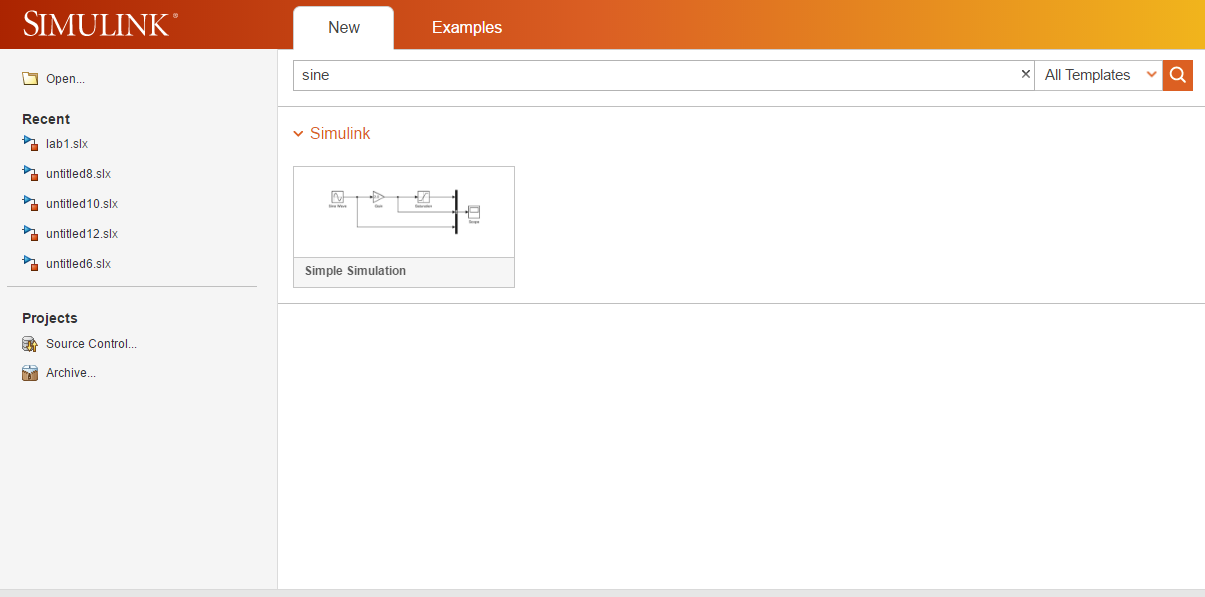
\includegraphics[width=1\linewidth]{img/000}}
\end{minipage}
\hfill
\begin{minipage}[h]{0.49\linewidth}
\center{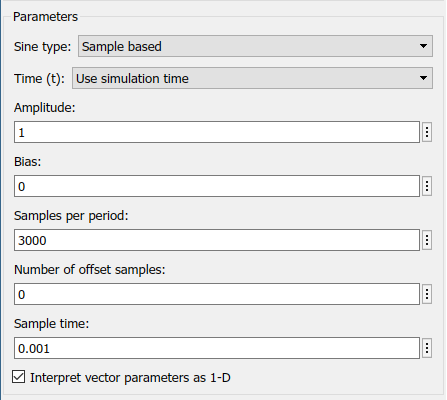
\includegraphics[width=1\linewidth]{img/001}}
\end{minipage}
\caption{Схема моделирующая синусоидальный сигнал}
\label{000}
\end{figure}

\begin{figure}[H]
\center{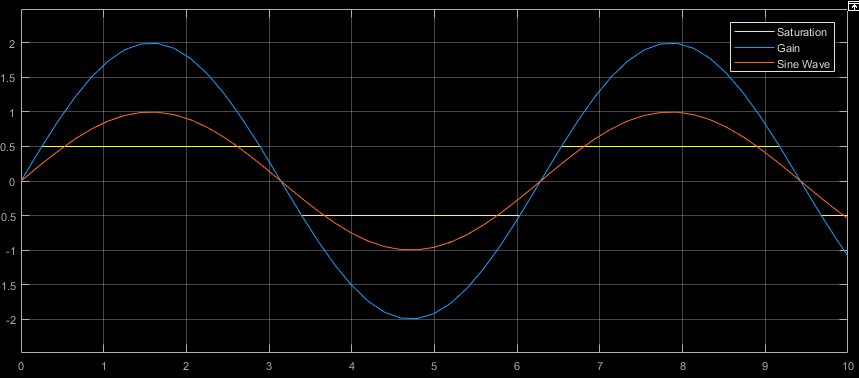
\includegraphics[width=1\linewidth]{img/002}}
\caption{Результат симуляции синтезированной схемы}
\label{002}
\end{figure}

\section{Амплитудная модуляция}

Схема с рисунка \ref{000} была модифицирована. Новая схема представлена на рисунке \ref{003}, а результат симуляции представлен на рисунке \ref{004}.

\begin{figure}[H]
\begin{minipage}[h]{0.69\linewidth}
\center{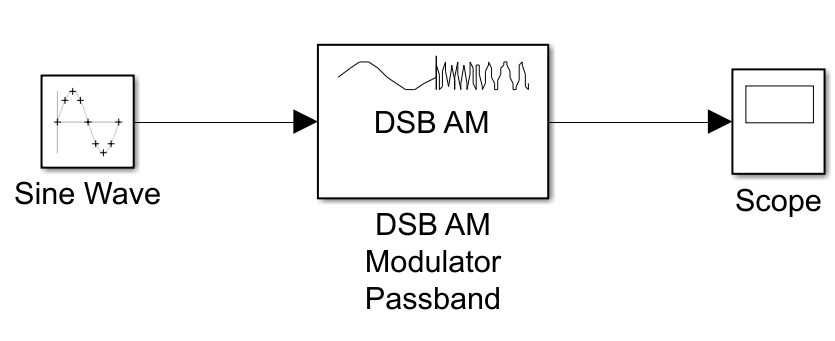
\includegraphics[width=1\linewidth]{img/003}}
\end{minipage}
\hfill
\begin{minipage}[h]{0.29\linewidth}
\center{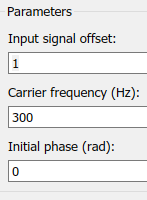
\includegraphics[width=0.7\linewidth]{img/202}}
\end{minipage}
\caption{Модифицированная схема для амплитудной модуляции}
\label{003}
\end{figure}

\begin{figure}[H]
\center{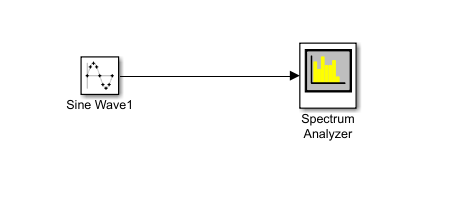
\includegraphics[width=1\linewidth]{img/004}}
\caption{Амплитудная модуляция}
\label{004}
\end{figure}

Чтобы снова получить информационный сигнал необходимо провести демодуляцию. На рисунке \ref{005} представлена модифицированная схема для демодуляции. Результат демодуляции представлен на рисунке \ref{006}, причём желтым цветом обозначен сигнал после демодуляции, а синим исходный сигнал.

\begin{figure}[H]
\center{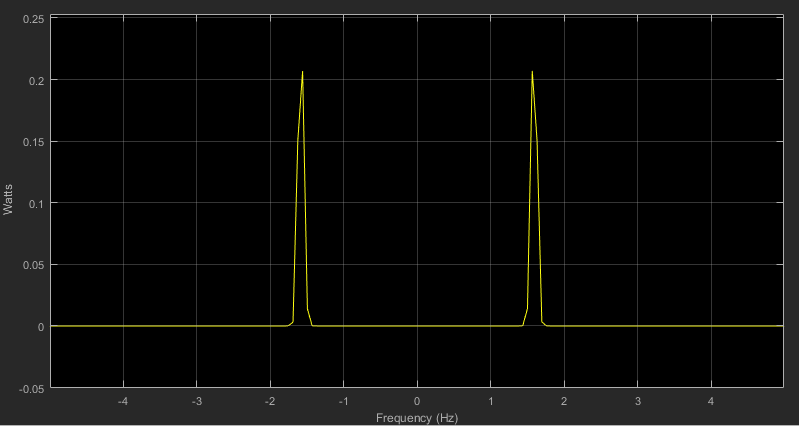
\includegraphics[width=1\linewidth]{img/005}}
\caption{Модифицированная схема для амплитудной демодуляции}
\label{005}
\end{figure}

\begin{figure}[H]
\center{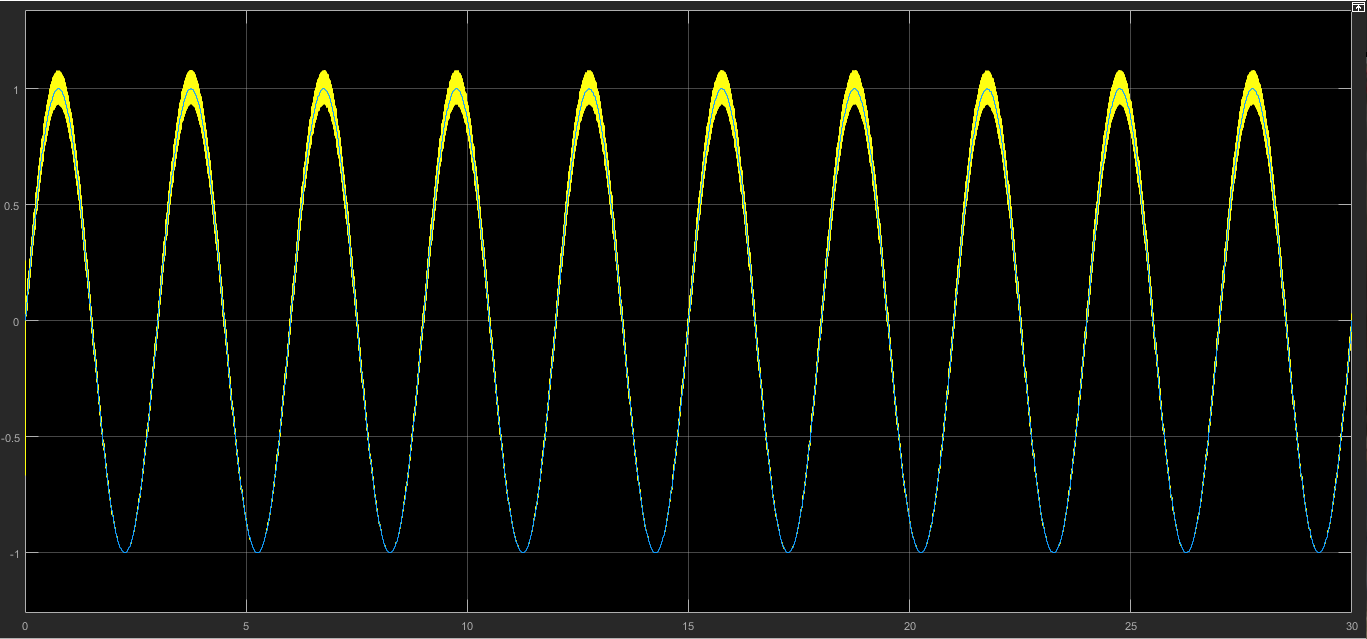
\includegraphics[width=1\linewidth]{img/006}}
\caption{Результат демодуляции}
\label{006}
\end{figure}

\begin{figure}[H]
\center{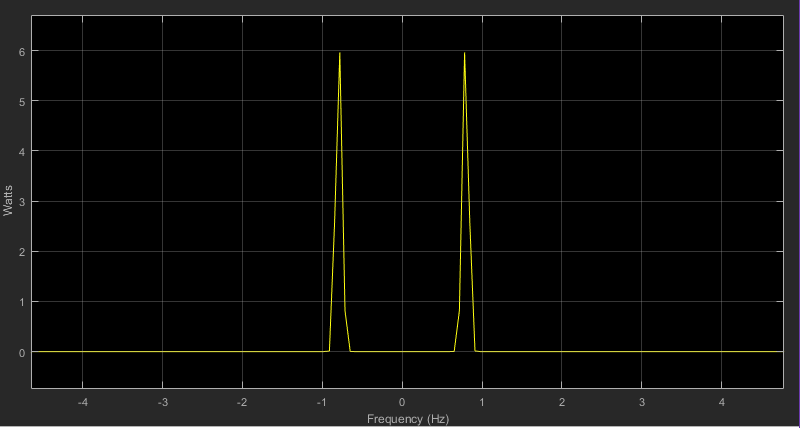
\includegraphics[width=1\linewidth]{img/007}}
\caption{Модифицированная схема с добавлением шума в канал передачи}
\label{007}
\end{figure}

\begin{figure}[H]
\center{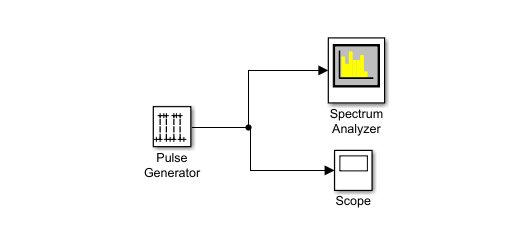
\includegraphics[width=0.625\linewidth]{img/008}}
\caption{Параметры устройства, добавляющего в канал передачи белый шум}
\label{008}
\end{figure}

\begin{figure}[H]
\center{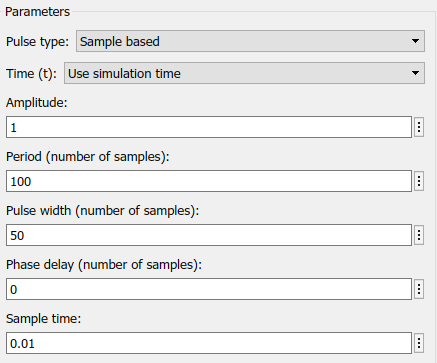
\includegraphics[width=0.9\linewidth]{img/009}}
\caption{Результат демодуляции после добавления в канал передачи шума}
\label{009}
\end{figure}

\begin{figure}[H]
\center{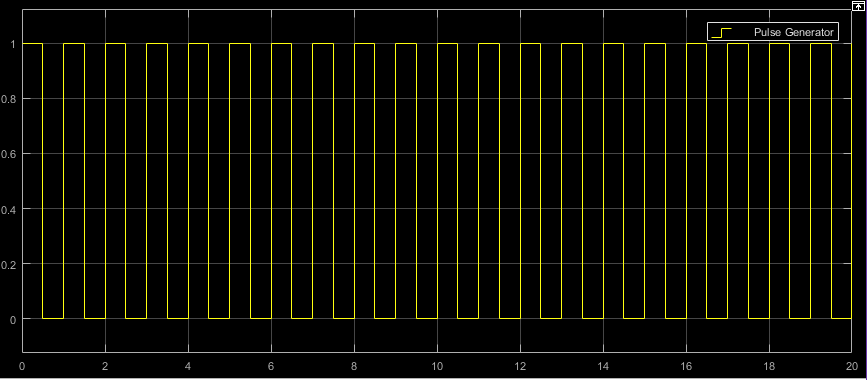
\includegraphics[width=0.9\linewidth]{img/010}}
\caption{Модифицированная схема для изучения спектра моделируемого сигнала}
\label{010}
\end{figure}

\begin{figure}[H]
\center{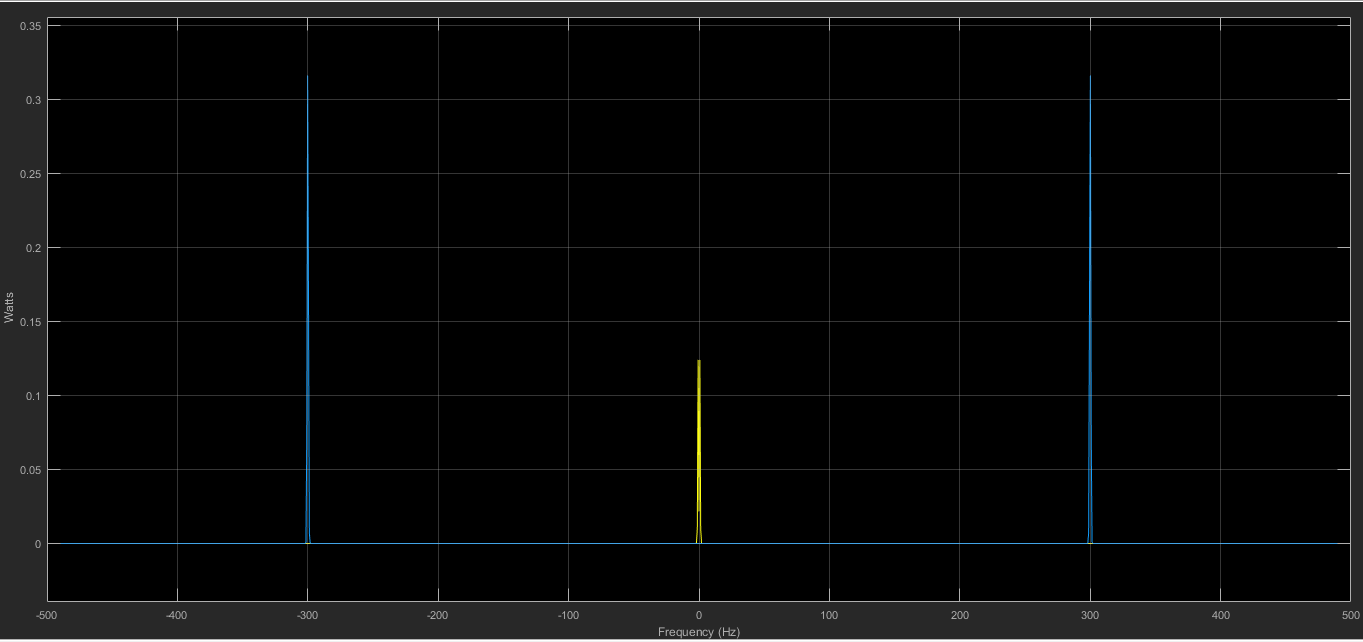
\includegraphics[width=0.8\linewidth]{img/304}}
\caption{Спектры моделированного и исходного сигнала выраженные в $Watts$}
\label{304}
\end{figure}

\begin{figure}[H]
\center{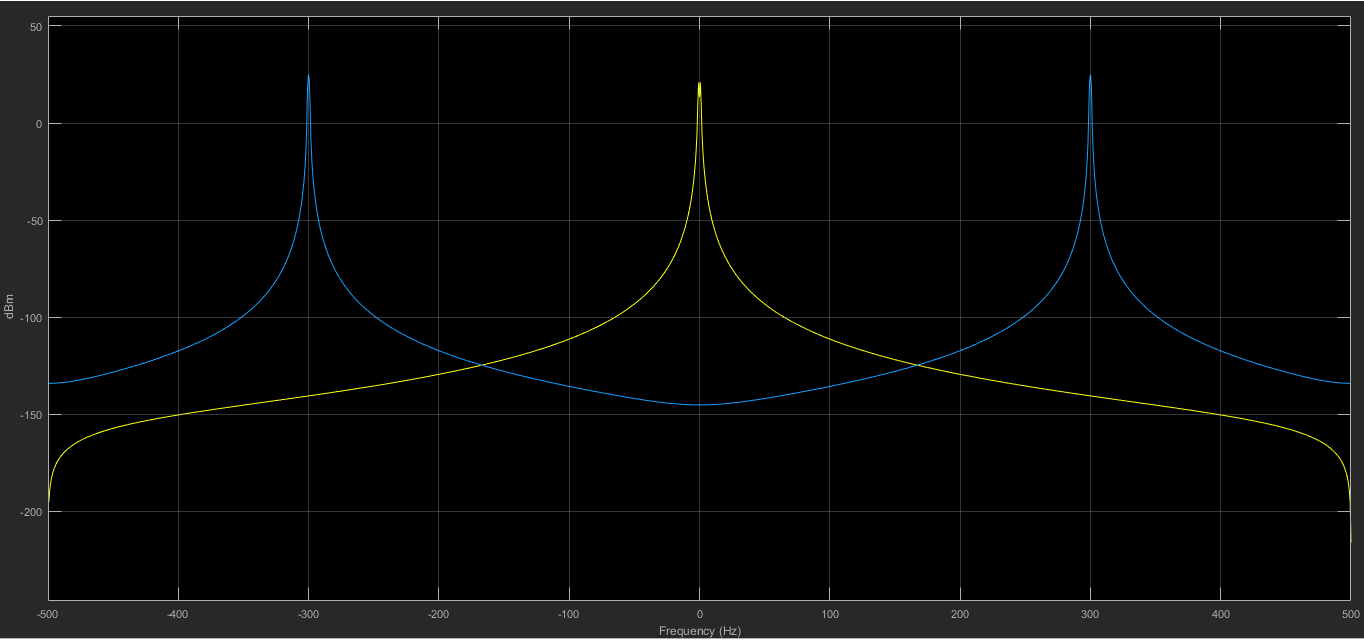
\includegraphics[width=0.82\linewidth]{img/305}}
\caption{Спектры моделированного и исходного сигнала выраженные в $dBm$}
\label{305}
\end{figure}

\begin{figure}[H]
\center{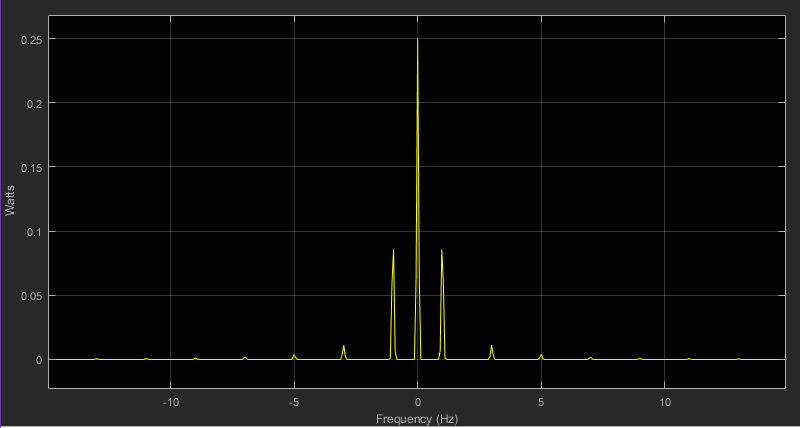
\includegraphics[width=0.82\linewidth]{img/011}}
\caption{Спектры демодулированного и исходного сигнала выраженные в $dBm$}
\label{011}
\end{figure}

\begin{figure}[H]
\center{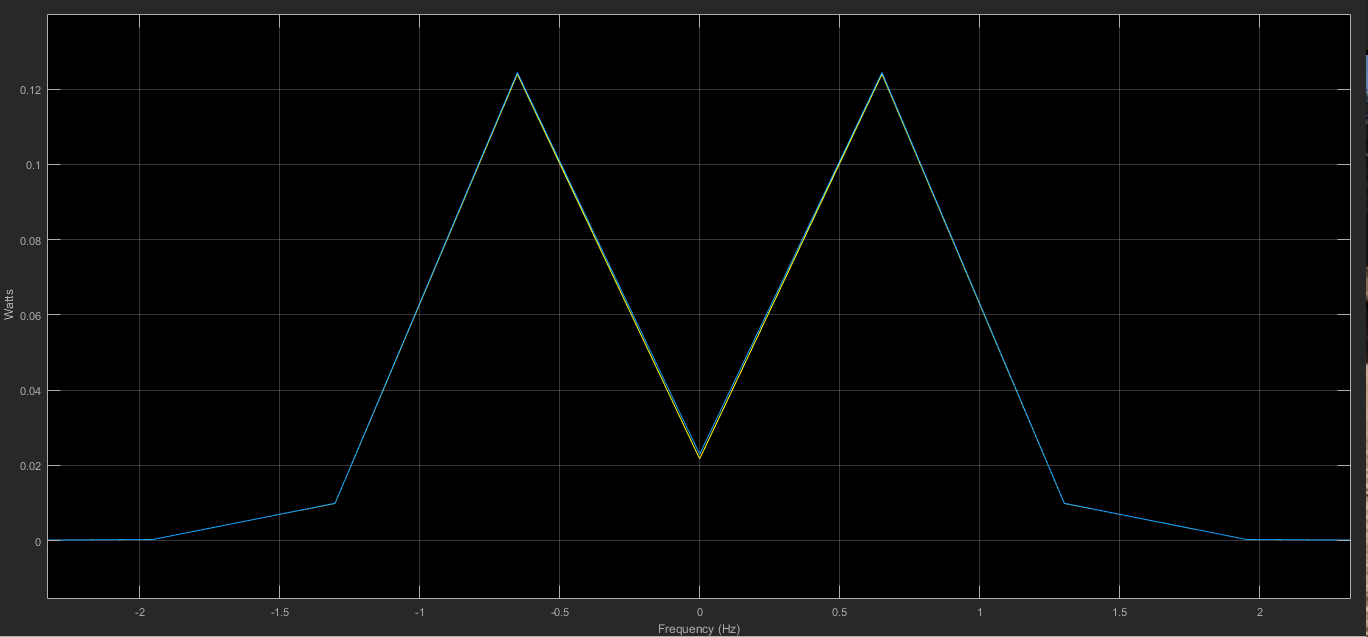
\includegraphics[width=0.82\linewidth]{img/012}}
\caption{Спектры демодулированного и исходного сигнала выраженные в $Watts$}
\label{012}
\end{figure}


\section{Частотная модуляция}

Модифицируем схему используемую для исследования амплитудной модуляции, представленную на рисунке \ref{010} для исследования частотной модуляции. Модифицированная схема представлена на рисунке \ref{014}.

\begin{figure}[H]
\begin{minipage}[h]{0.69\linewidth}
\center{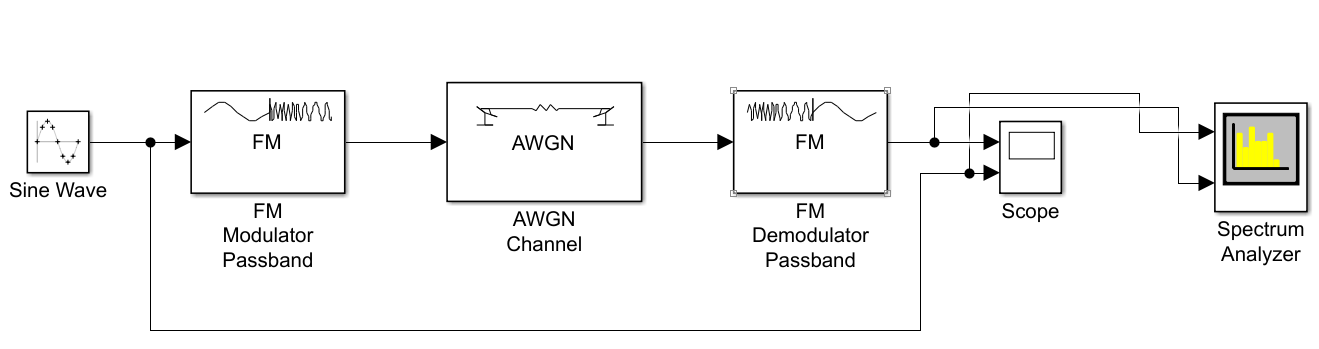
\includegraphics[width=1\linewidth]{img/014}}
\end{minipage}
\hfill
\begin{minipage}[h]{0.29\linewidth}
\center{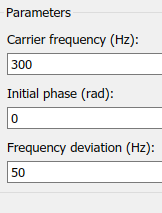
\includegraphics[width=0.7\linewidth]{img/201}}
\end{minipage}
\caption{Модифицированная схема для исследования частотной модуляции}
\label{014}
\end{figure}

\begin{figure}[H]
\center{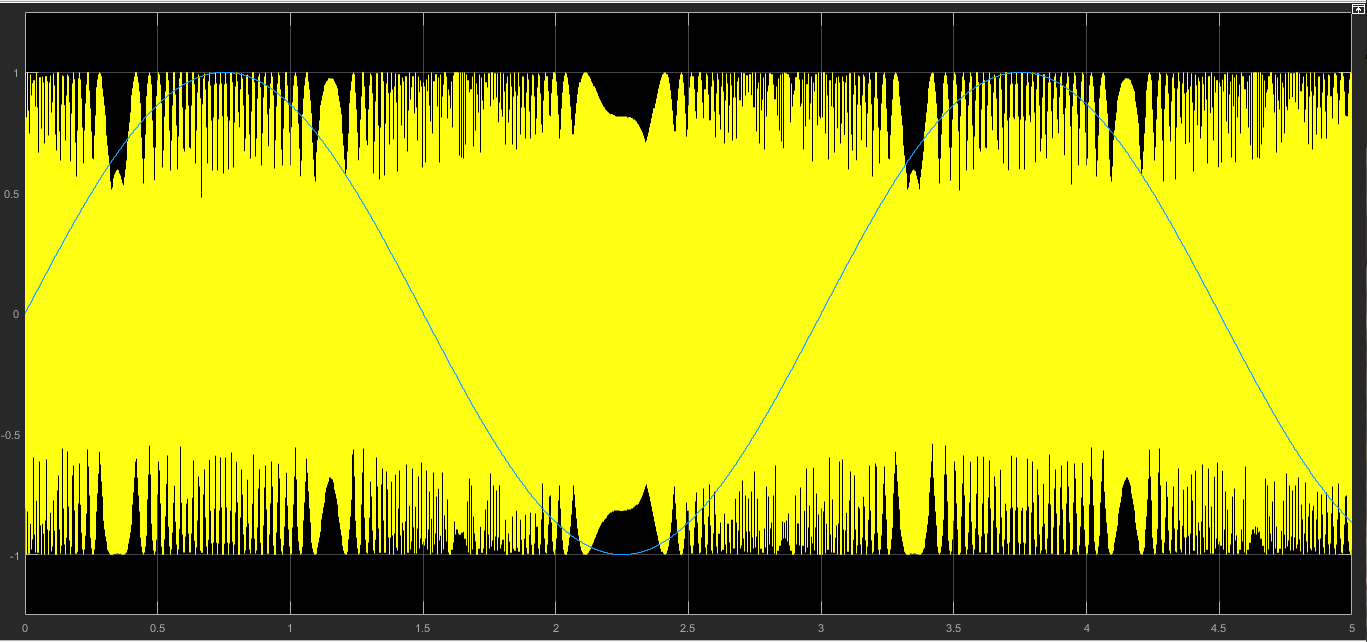
\includegraphics[width=0.8\linewidth]{img/015}}
\caption{Результат частотной модуляции синусоидального сигнала}
\label{015}
\end{figure}

\begin{figure}[H]
\center{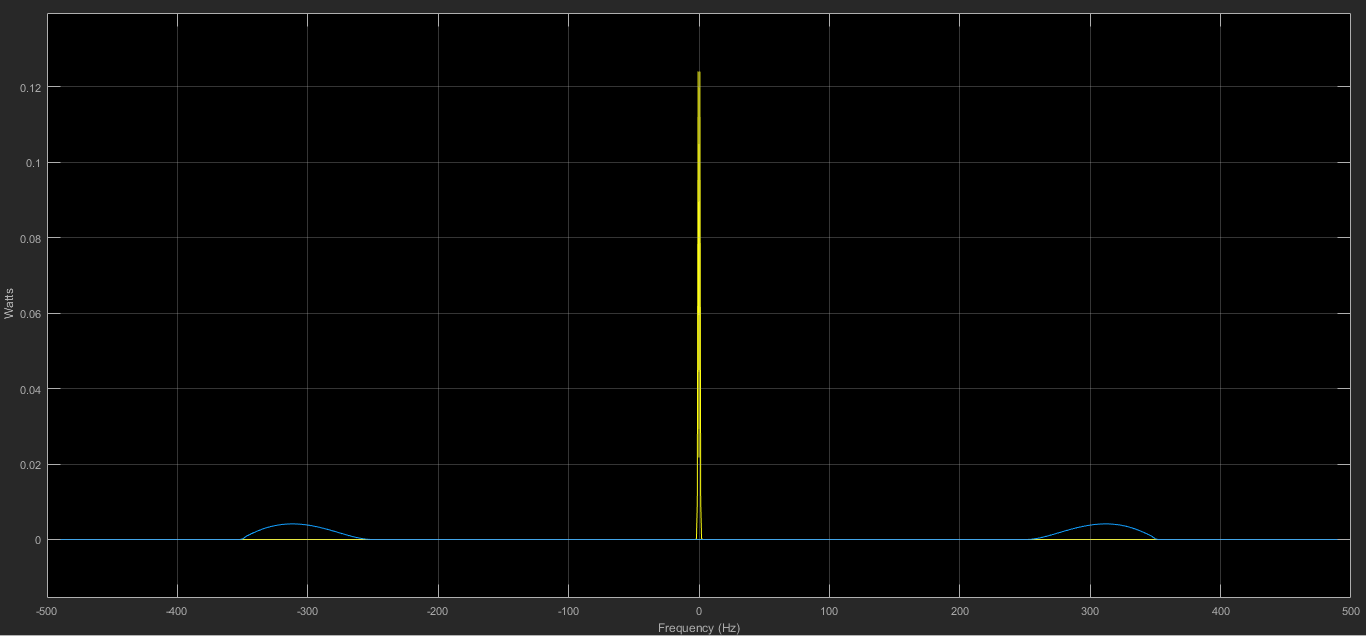
\includegraphics[width=0.8\linewidth]{img/302}}
\caption{Спектры моделированного и исходного сигнала выраженные в $Watts$}
\label{302}
\end{figure}

\begin{figure}[H]
\center{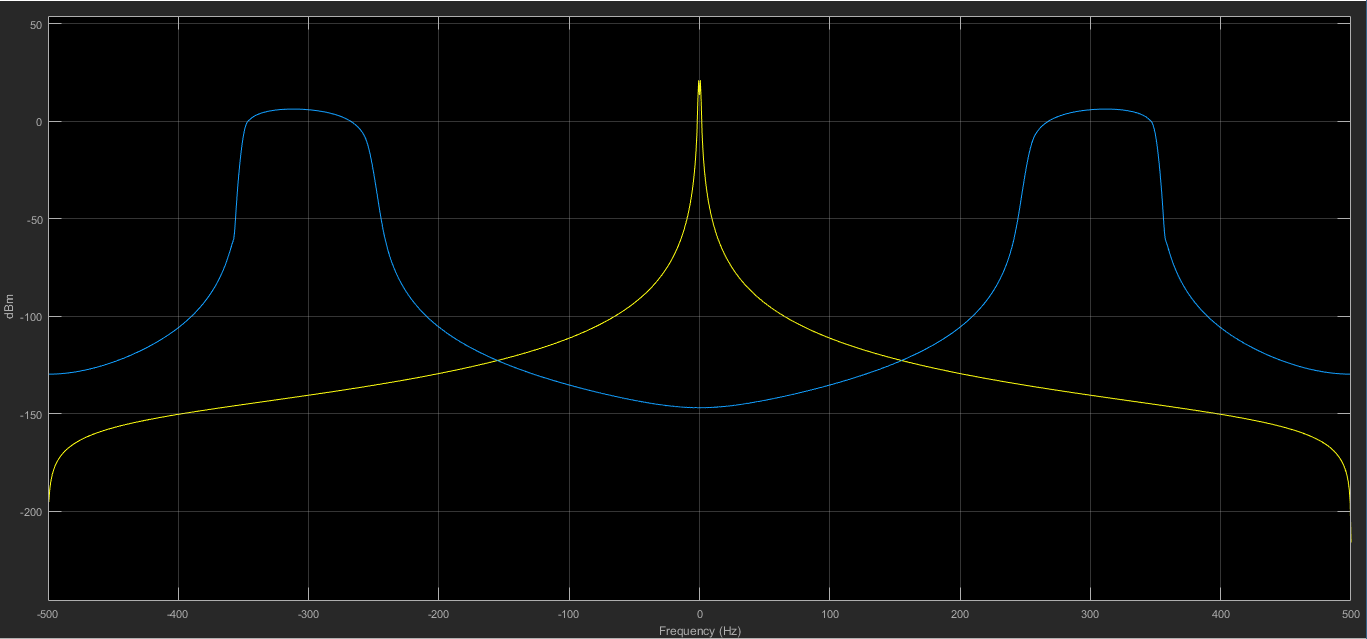
\includegraphics[width=0.88\linewidth]{img/303}}
\caption{Спектры моделированного и исходного сигнала выраженные в $dBm$}
\label{303}
\end{figure}

\begin{figure}[H]
\center{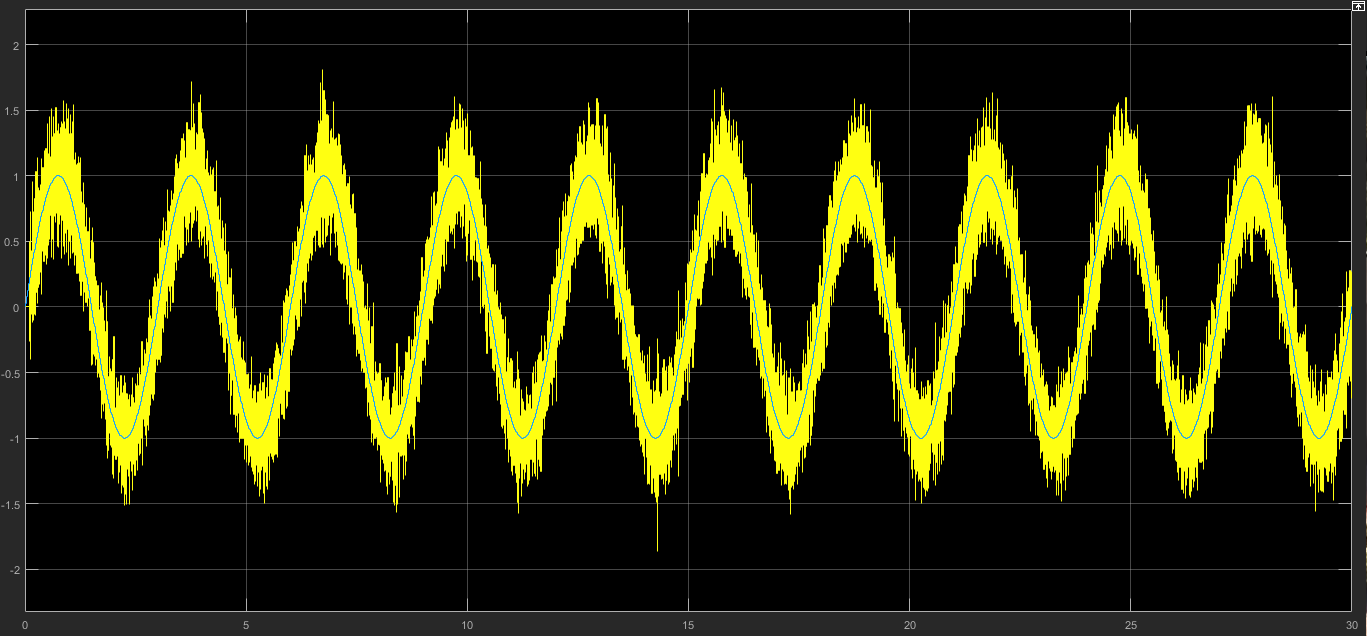
\includegraphics[width=0.85\linewidth]{img/016}}
\caption{Результат демодуляции}
\label{016}
\end{figure}

\begin{figure}[H]
\center{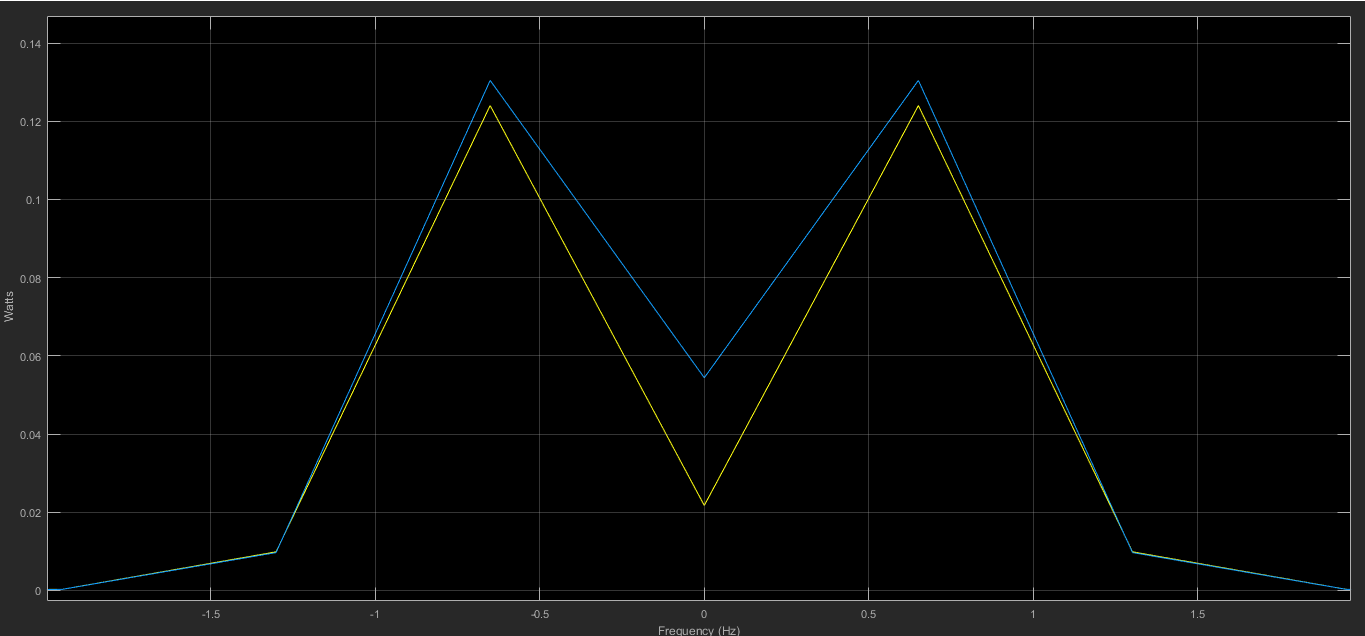
\includegraphics[width=0.85\linewidth]{img/017}}
\caption{Спектры демодулированного и исходного сигнала выраженные в $dBm$}
\label{017}
\end{figure}

\begin{figure}[H]
\center{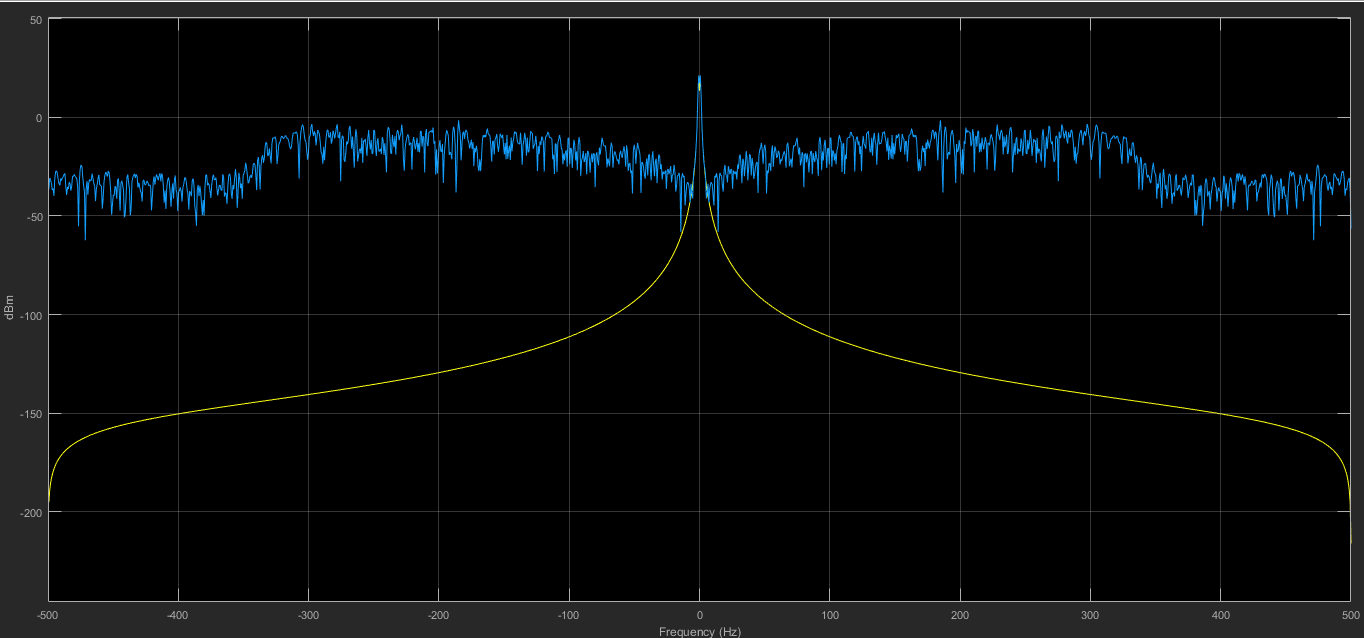
\includegraphics[width=0.85\linewidth]{img/018}}
\caption{Спектры демодулированного и исходного сигнала выраженные в $Watts$}
\label{018}
\end{figure}

\section{Фазовая модуляция}

Модифицируем схему используемую для исследования частотной модуляции, представленную на рисунке \ref{014} для исследования фазовой модуляции. Модифицированная схема представлена на рисунке \ref{019}.

\begin{figure}[H]
\begin{minipage}[h]{0.69\linewidth}
\center{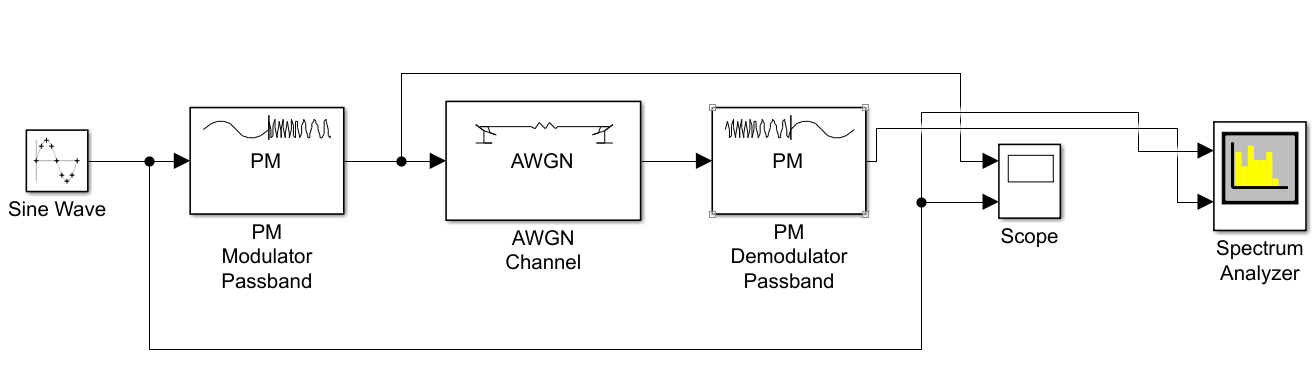
\includegraphics[width=1\linewidth]{img/019}}
\end{minipage}
\hfill
\begin{minipage}[h]{0.29\linewidth}
\center{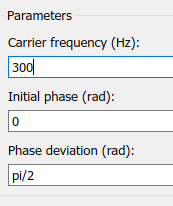
\includegraphics[width=0.7\linewidth]{img/200}}
\end{minipage}
\caption{Модифицированная схема для исследования фазовой модуляции}
\label{019}
\end{figure}

\begin{figure}[H]
\center{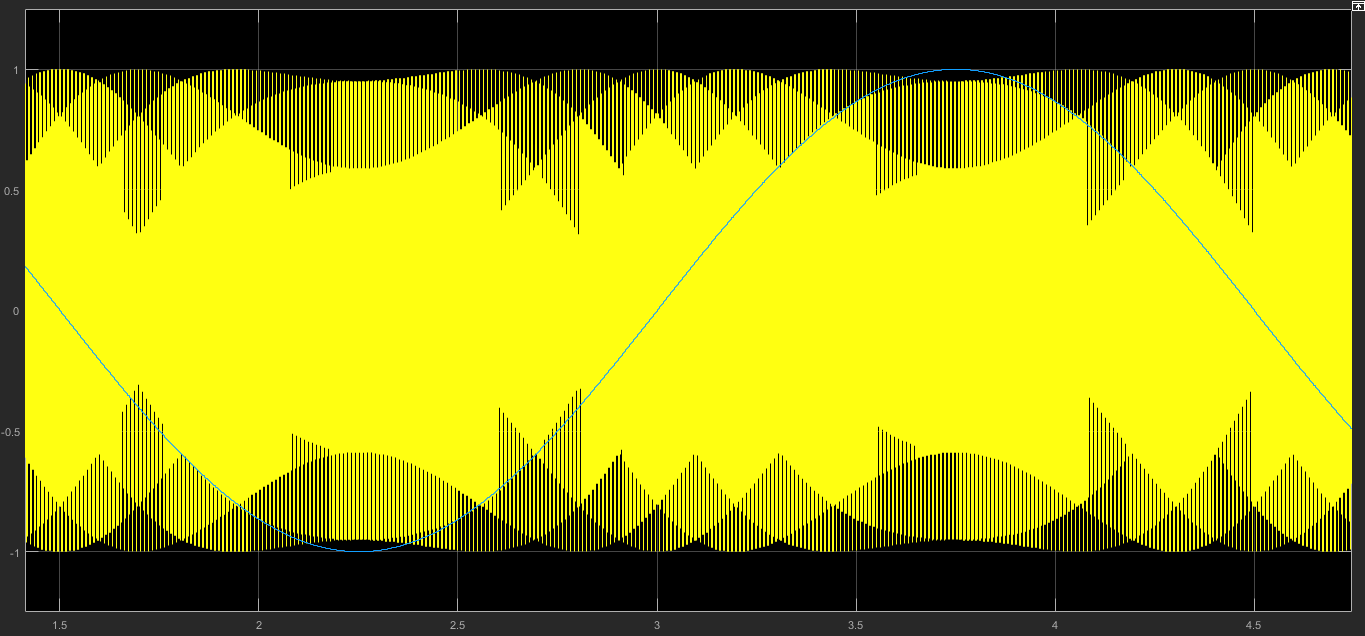
\includegraphics[width=0.8\linewidth]{img/020}}
\caption{Результат частотной модуляции синусоидального сигнала}
\label{020}
\end{figure}

\begin{figure}[H]
\center{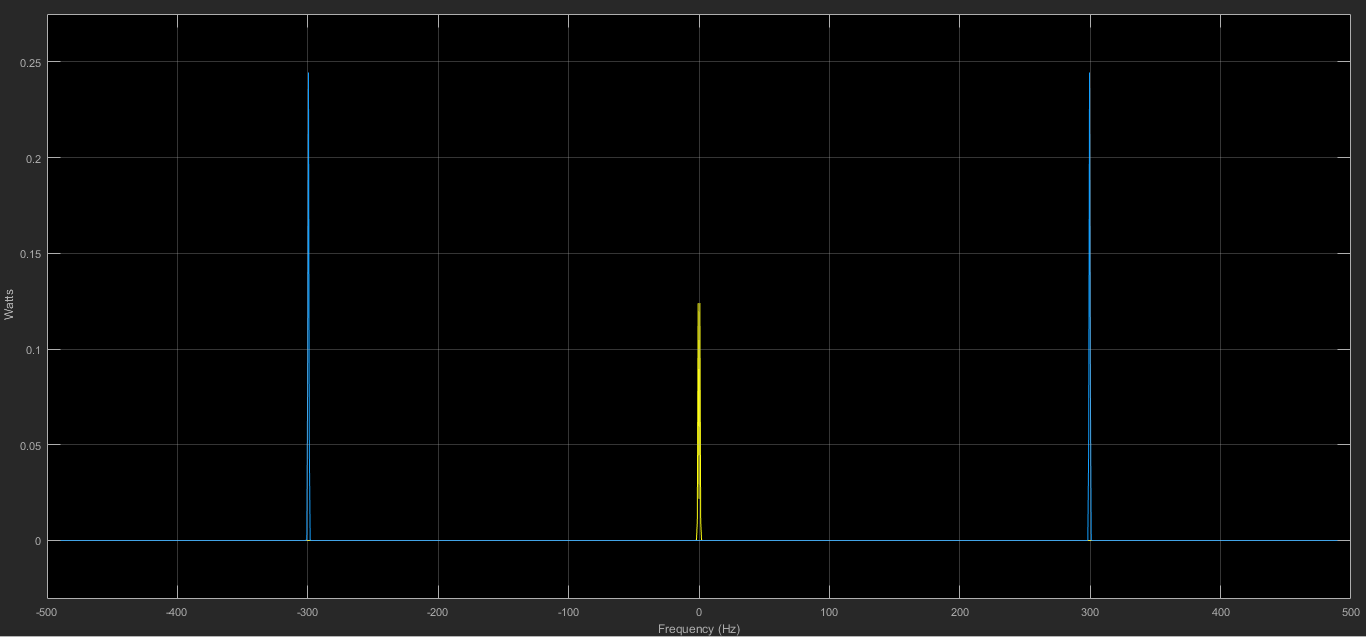
\includegraphics[width=0.8\linewidth]{img/300}}
\caption{Спектры моделированного и исходного сигнала выраженные в $Watts$}
\label{300}
\end{figure}

\begin{figure}[H]
\center{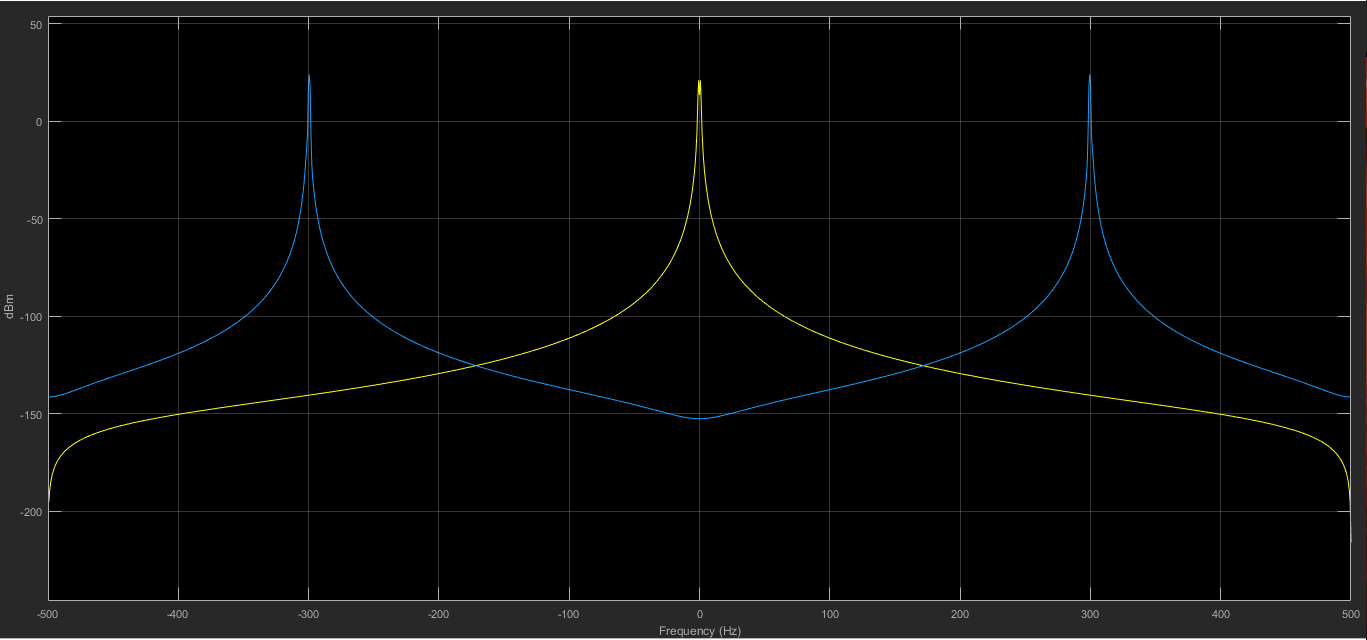
\includegraphics[width=0.88\linewidth]{img/301}}
\caption{Спектры моделированного и исходного сигнала выраженные в $dBm$}
\label{301}
\end{figure}

\begin{figure}[H]
\center{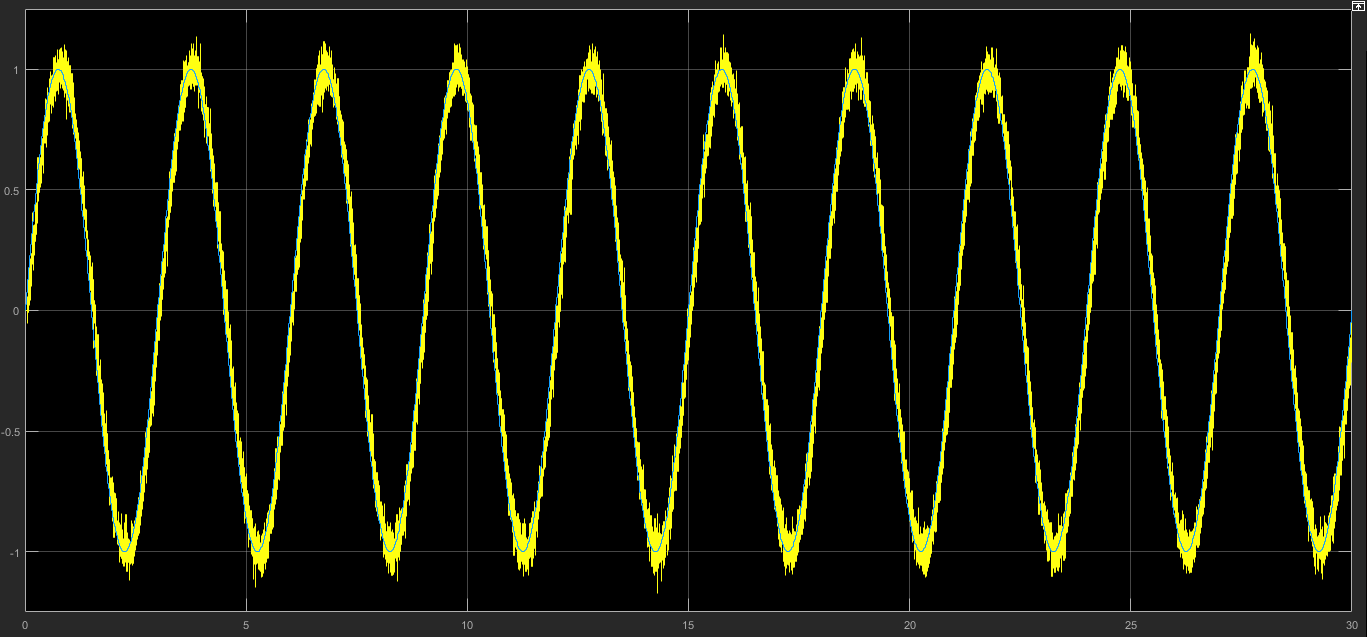
\includegraphics[width=0.85\linewidth]{img/021}}
\caption{Результат демодуляции}
\label{021}
\end{figure}

\begin{figure}[H]
\center{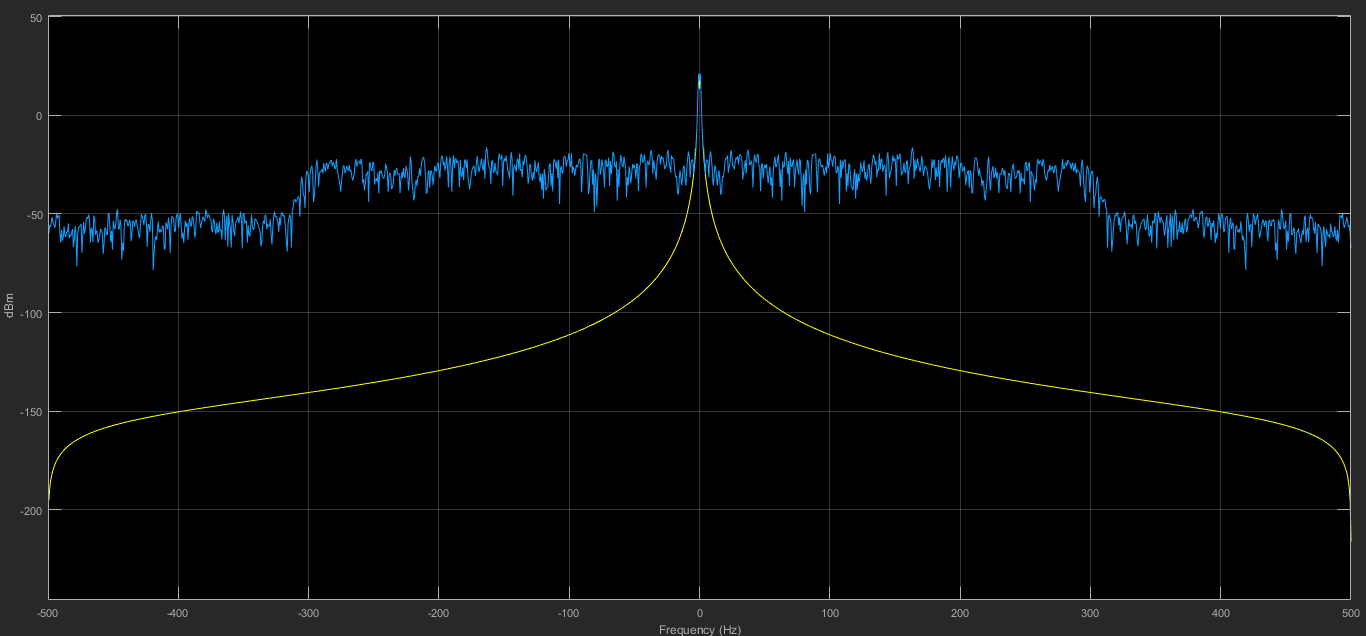
\includegraphics[width=0.85\linewidth]{img/022}}
\caption{Спектры демодулированного и исходного сигнала выраженные в $dBm$}
\label{022}
\end{figure}

\begin{figure}[H]
\center{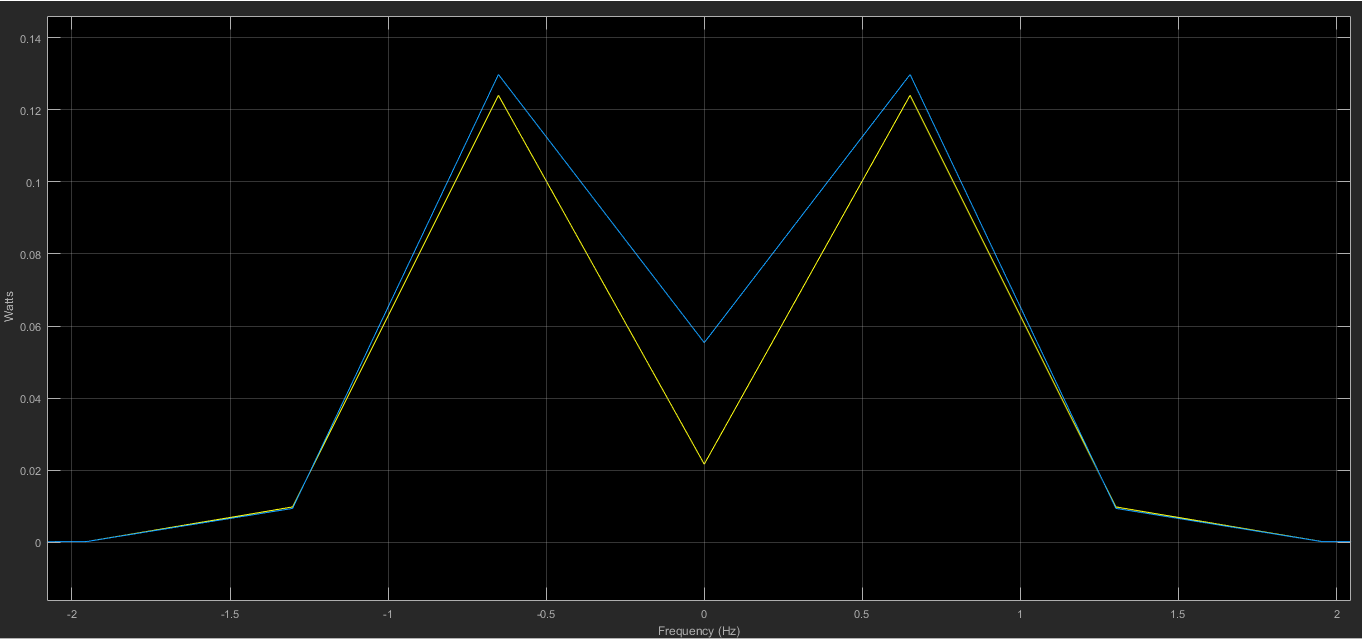
\includegraphics[width=0.85\linewidth]{img/023}}
\caption{Спектры демодулированного и исходного сигнала выраженные в $Watts$}
\label{023}
\end{figure}

\section{Выводы}

Модуляция позволяет передавать информационные сигналы на большие расстояния. Она делится на:

\begin{itemize}
\item Амплитудная модуляция

Помехонеустойчивость возникает вследствие узкой полосы модулируемого сигнала. Ее используют в основном в средне- и низкочастотных интервалах электромагнитного спектра.

\item Частотная модуляция

Такая модуляция характеризуется высокой помехоустойчивостью, однако для ее применения следует использовать высокочастотный диапазон.

\item Фазовая модуляция

Фазовая модуляция активно используется для формирования помехозащищенной связи в микроволновом диапазоне.
\end{itemize}

\section{Используемые материалы}

\begin{enumerate}
\item \href{https://en.wikipedia.org/wiki/Modulation}{Modulation (Wikipedia)}
\item \href{https://www.intuit.ru/studies/courses/1004/202/lecture/5236?page=3}{Лекция 1: Организация беспроводных сетей (стр. 3)}
\item \href{https://refdb.ru/look/1101001.html}{Лекция №9 Модуляция сигналов}
\item \href{http://conture.by/post/422}{Что такое модуляция и разновидности модулированных сигналов?}
\end{enumerate}

\end{document}